\documentclass[12pt,a4paper]{article}

% --- Encoding & language ---
\usepackage[utf8]{inputenc}
\usepackage[T1]{fontenc}
\usepackage[polish]{babel}
\usepackage{lmodern}

% --- Math & symbols ---
\usepackage{amsmath,amssymb,amsthm}
\usepackage{mathtools}
\usepackage{bm}

% --- Layout ---
\usepackage[margin=2.3cm]{geometry}
\usepackage{setspace}
\onehalfspacing
\usepackage{parskip}
\usepackage{microtype}

% --- Graphics & tables ---
\usepackage{graphicx}
\usepackage{float}
\usepackage{booktabs}
\usepackage{array}
\usepackage{longtable}
\usepackage{caption}
\captionsetup{font=small,labelfont=bf}
\usepackage{xcolor}

% --- Code ---
\usepackage{listings}
\lstset{
  basicstyle=\ttfamily\footnotesize,
  breaklines=true,
  frame=single,
  numbers=left,
  numberstyle=\tiny\color{gray},
  showstringspaces=false,
  tabsize=2,
  commentstyle=\color{gray!70!black},
  keywordstyle=\color{blue!60!black}\bfseries,
  stringstyle=\color{green!50!black},
  language=Python
}

% --- Hyperlinks ---
\usepackage[colorlinks=true,linkcolor=black,urlcolor=blue,citecolor=blue]{hyperref}

% --- Header / footer ---
\usepackage{fancyhdr}
\pagestyle{fancy}
\fancyhf{}
\fancyhead[L]{\small \textit{Modele klasyfikacji: regresja logistyczna na danych klinicznych}}
\fancyfoot[C]{\thepage}
\renewcommand{\headrulewidth}{0.4pt}

% --- Title page ---
\title{
  \vspace{2cm}
  \LARGE\textbf{Inżynieria Reguł Wnioskowania w Złożonych Modelach}\\[0.6cm]
  \Large Laboratorium 2\\[0.4cm]
  \large \textit{Modele klasyfikacji: regresja logistyczna na danych klinicznych}\\[0.3cm]
  \normalsize Wariant: \textbf{1 (fallback z 8) — klasyfikacja przeżycia (prostate cancer)}
}
\author{Jakub Jurzak 59099}
\date{07.05.2026}

\begin{document}
\maketitle
\thispagestyle{empty}
\newpage

\tableofcontents
\newpage

\section{Cel zadania}
Budowa i ewaluacja prostego modelu klasyfikacyjnego (regresja logistyczna) rozpoznającego stan kliniczny pacjenta na podstawie danych z lab1 (syntetyczna kohorta prostate cancer).

\section{Opis problemu}
Predykcja przeżycia pacjenta (\texttt{survived}=1) na bazie cech: \texttt{age}, \texttt{psa}, \texttt{gleason\_score}, \texttt{comorbidities}, \texttt{tumor\_stage}, \texttt{treatment}. Klasy są niezbalansowane — stosujemy \texttt{class\_weight=balanced}.

\section{Opis danych}
Zbiór z lab1: \texttt{prostate\_cancer\_synth.csv} ($N=600$). Braki w kolumnie \texttt{psa} uzupełniono medianą. Cechy kategoryczne zakodowano OHE (drop first). Wszystkie cechy ilościowe wystandaryzowane (\texttt{StandardScaler}).

\section{Opis metod}
Regresja logistyczna z regularyzacją L2 (\texttt{lbfgs}, \texttt{max\_iter}=2000) i wagami klas. Podział train/test 75/25 ze stratyfikacją po etykiecie. Miary: accuracy, precision, recall, F1, ROC AUC. Diagnostyka: krzywa ROC, krzywa PR, macierz pomyłek, ranking współczynników.

\section{Opis implementacji}
Plik \texttt{lab2/lab2\_solution.py}. Funkcje \texttt{prepare}, \texttt{evaluate}, \texttt{plot\_*} oraz \texttt{main} oddzielają etapy preprocessingu, treningu, ewaluacji i wizualizacji. Brak hardkodów, ścieżki względne.

\section{Obliczenia}
Pomocnicze obliczenie odds ratio dla każdej cechy: $\text{OR}_j = \exp(\beta_j)$. Dla cech wystandaryzowanych $\beta_j$ interpretujemy jako efekt zmiany o jedno odchylenie standardowe.

\begin{table}[H]
\centering
\begin{tabular}{lrr}
\toprule
cecha & współczynnik & odds\_ratio \\
\midrule
treatment\_surgery & 0.1190 & 1.1270 \\
comorbidities & -0.0190 & 0.9810 \\
treatment\_radiation & -0.0520 & 0.9490 \\
tumor\_stage\_T2 & -0.1330 & 0.8750 \\
tumor\_stage\_T4 & -0.2930 & 0.7460 \\
psa & -0.3230 & 0.7240 \\
treatment\_watch & -0.4260 & 0.6530 \\
age & -0.4440 & 0.6410 \\
tumor\_stage\_T3 & -0.4900 & 0.6120 \\
gleason\_score & -0.8450 & 0.4300 \\
\bottomrule
\end{tabular}

\caption{Współczynniki regresji logistycznej i odds ratio.}
\label{tab:coef}
\end{table}


\section{Wyniki}
Miary jakości na zbiorze testowym ($N_{test}=150$):

\begin{table}[H]
\centering
\begin{tabular}{lr}
\toprule
miara & wartość \\
\midrule
accuracy & 0.740 \\
precision & 0.933 \\
recall & 0.754 \\
F1 & 0.834 \\
ROC AUC & 0.754 \\
\bottomrule
\end{tabular}

\caption{Miary jakości klasyfikacji.}
\label{tab:metrics}
\end{table}


\section{Wykresy}
\begin{figure}[H]
\centering
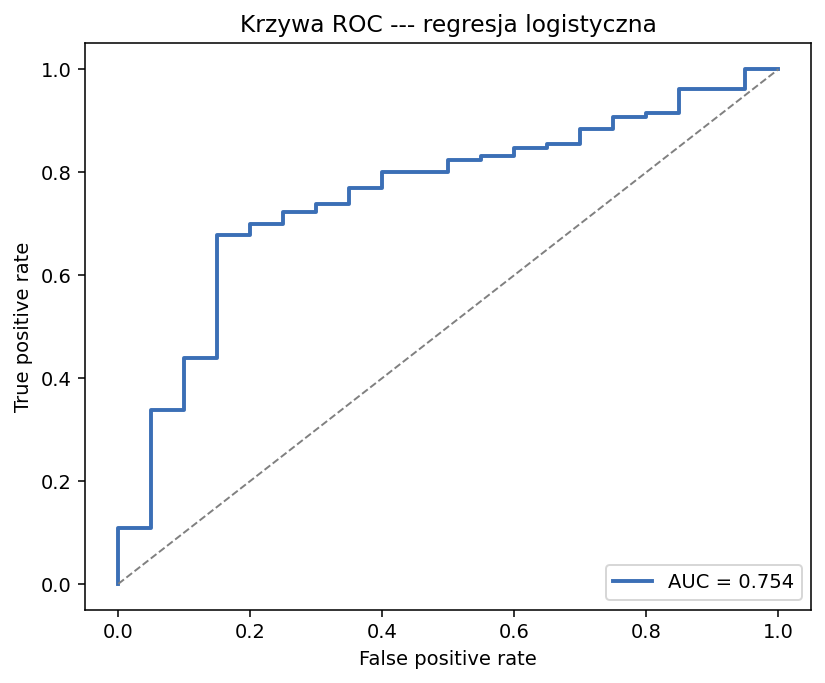
\includegraphics[width=0.85\linewidth]{roc.png}
\caption{Krzywa ROC.}
\label{fig:roc}
\end{figure}
\begin{figure}[H]
\centering
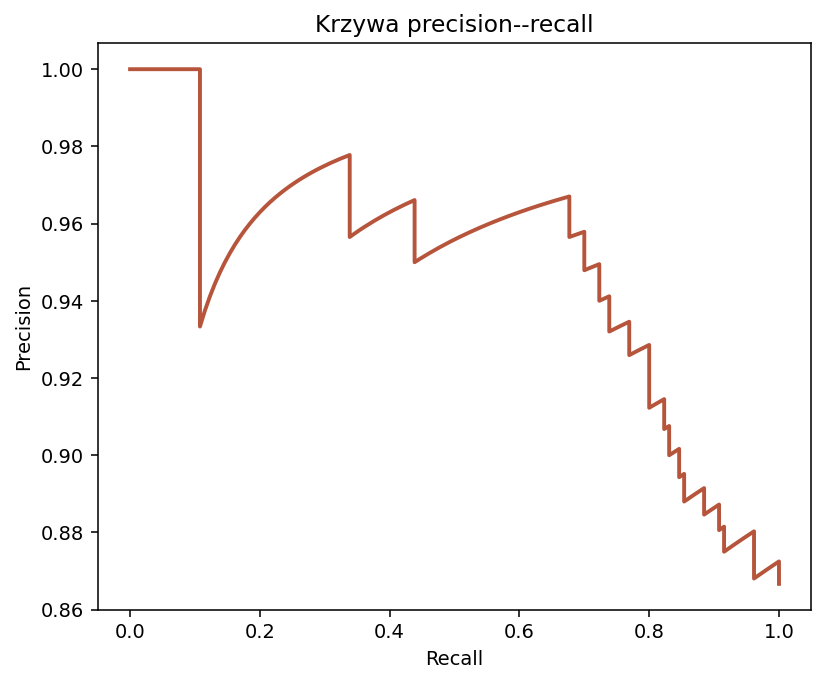
\includegraphics[width=0.85\linewidth]{pr.png}
\caption{Krzywa precision-recall.}
\label{fig:pr}
\end{figure}
\begin{figure}[H]
\centering
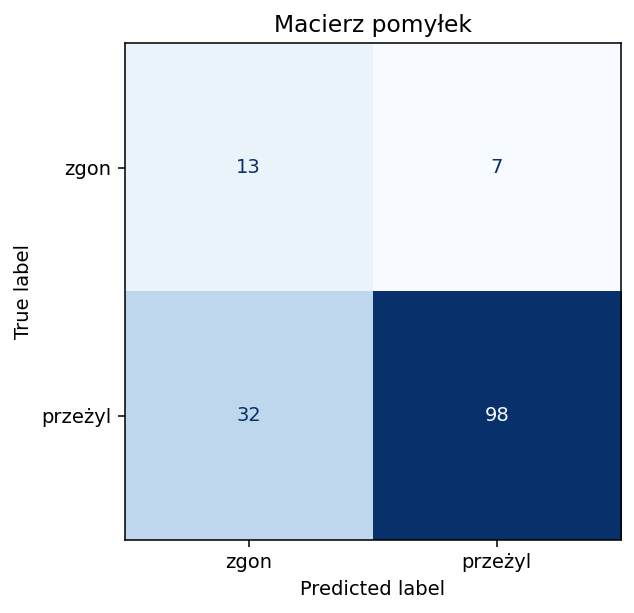
\includegraphics[width=0.85\linewidth]{cm.png}
\caption{Macierz pomyłek.}
\label{fig:cm}
\end{figure}
\begin{figure}[H]
\centering
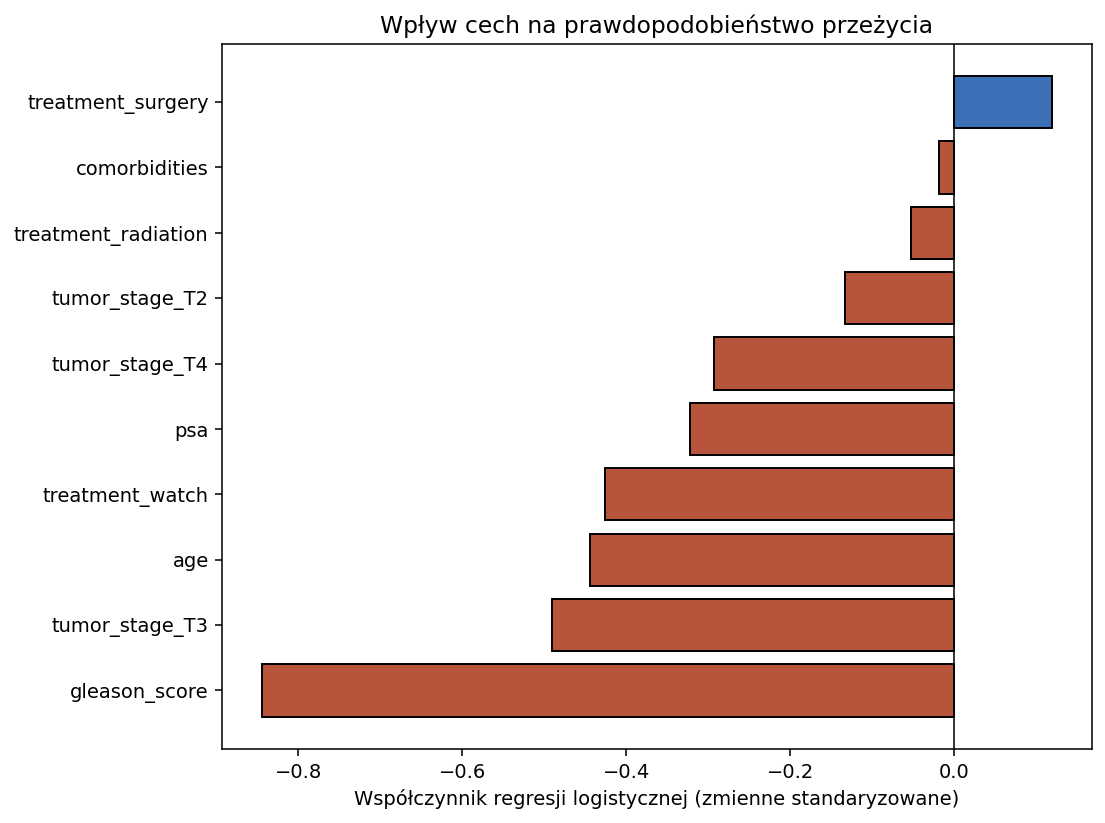
\includegraphics[width=0.85\linewidth]{coefs.png}
\caption{Współczynniki regresji logistycznej.}
\label{fig:coefs}
\end{figure}


\section{Interpretacja wyników}
Model osiąga ROC AUC = 0.754, F1 = 0.834, co świadczy o zauważalnej zdolności separacji klas. Ranking współczynników wskazuje, że Gleason score, PSA i wiek pacjenta zwiększają ryzyko zgonu (ujemny wpływ na \texttt{survived}=1), natomiast leczenie operacyjne i radioterapia wpływają korzystnie. Krzywa precision-recall potwierdza, że dobór progu decyzyjnego może istotnie zmieniać kompromis między wykrywalnością a precyzją.

\section{Wnioski}
Regresja logistyczna na omawianym zbiorze stanowi solidną linię bazową: interpretowalna (wagi i OR), szybka, dobrze skalibrowana po standaryzacji. Aby poprawić jakość warto rozważyć: (a) modele drzewiaste (np. random forest, gradient boosting) — następne ćwiczenia; (b) dodatkowe cechy z domeny klinicznej; (c) optymalizację progu klasyfikacji pod konkretną miarę kliniczną.

\end{document}
